% CVPR 2027 Paper Template; see https://github.com/cvpr-org/author-kit

\documentclass[10pt,twocolumn,letterpaper]{article}

%%%%%%%%% PAPER TYPE  - PLEASE UPDATE FOR FINAL VERSION
% \usepackage{cvpr}              % To produce the CAMERA-READY version
\usepackage[review]{cvpr}      % To produce the REVIEW version
% \usepackage[pagenumbers]{cvpr} % To force page numbers, e.g. for an arXiv version

% Import additional packages in the preamble file, before hyperref
%% This file contains a number of tweaks that are typically applied to the main document.
%% They are not enabled by default, but can be enabled by uncommenting the relevant lines.
\usepackage{placeins}

%%
%% Inline annotations; for predefined colors, refer to "dvipsnames" in the xcolor package:
%% https://tinyurl.com/overleaf-colors
%%
\newcommand{\red}[1]{{\color{red}#1}}
\newcommand{\todo}[1]{{\color{red}#1}}
\newcommand{\TODO}[1]{\textbf{\color{red}[TODO: #1]}}
%%
%% disable for camera ready / submission by uncommenting these lines  
%%
% \renewcommand{\TODO}[1]{}
% \renewcommand{\todo}[1]{#1}

%%
%% work harder in optimizing text layout. Typically shrinks text by 1/6 of page, enable
%% it at the very end of the writing process, when you are just above the page limit
%%
% \usepackage{microtype}

%%
%% fine-tune paragraph spacing
%%
% \renewcommand{\paragraph}[1]{\vspace{.5em}\noindent\textbf{#1.}}

%%
%% globally adjusts space between figure and caption
%%
% \setlength{\abovecaptionskip}{.5em}


%%
%% Allows "the use of \paper to refer to the project name"
%% with automatic management of space at the end of the word
%%
% \usepackage{xspace}
% \newcommand{\paper}{ProjectName\xspace}

%%
%% Commonly used math definitions
%%
% \DeclareMathOperator*{\argmin}{arg\,min}
% \DeclareMathOperator*{\argmax}{arg\,max}

%%
%% Tigthen underline
%%
% \usepackage{soul}
% \setuldepth{foobar}


% It is strongly recommended to use hyperref, especially for the review version.
% hyperref with option pagebackref eases the reviewers' job.
% Please disable hyperref *only* if you encounter grave issues, 
% e.g. with the file validation for the camera-ready version.
%
% If you comment hyperref and then uncomment it, you should delete *.aux before re-running LaTeX.
% (Or just hit 'q' on the first LaTeX run, let it finish, and you should be clear).
\definecolor{cvprblue}{rgb}{0.21,0.49,0.74}
\usepackage[pagebackref,breaklinks,colorlinks,allcolors=cvprblue]{hyperref}

\def\confName{CVPR}
\def\confYear{2027}

%%%%%%%%% TITLE - PLEASE UPDATE
\title{Detect and Suppress: Safe Text-to-Image Generation via Learned Prompt Pairs}

%%%%%%%%% AUTHORS - PLEASE UPDATE
\author{First Author\\
Institution1\\
Institution1 address\\
{\tt\small firstauthor@i1.org}
% For a paper whose authors are all at the same institution,
% omit the following lines up until the closing ``}''.
% Additional authors and addresses can be added with ``\and'',
% just like the second author.
% To save space, use either the email address or home page, not both
\and
Second Author\\
Institution2\\
First line of institution2 address\\
{\tt\small secondauthor@i2.org}
}

\begin{document}
\maketitle

\begin{abstract}
Text-to-image diffusion models can generate harmful content and reproduce unwanted visual concepts, motivating concept erasure that removes designated concepts while preserving benign generation.
Existing approaches can alter unrelated content through weight editing or indiscriminate intervention, while manually written negative prompts often fail to suppress target concepts. To tackle these issues, 
we introduce \textbf{Detect and Suppress (DAS)}, a framework that decouples when to intervene from how to suppress target concepts.
For each concept, DAS independently learns a detection prompt to identify relevant inputs and a suppression prompt to steer generation through the negative branch of classifier-free guidance.
The detection prompt combines text discrimination with visual reconstruction, while the suppression prompt is trained to align guided predictions with those of safe reference prompts.
At inference, detection runs once before sampling and activates the paired suppression prompt only for identified inputs; other inputs retain their original sampling process.
Both the text encoders and the generative model remain frozen throughout training and inference.
Experiments on the modern Diffusion Transformer-based Stable Diffusion 3.5 across NSFW content, IP characters, artistic styles, and objects show that DAS outperforms existing methods in balancing concept suppression and benign generation preservation.
\end{abstract}

\section{Introduction}
\label{sec:intro}

Text-to-image diffusion models learn a denoising process conditioned on natural-language descriptions, predicting how to recover a clean image from noise~\cite{NEURIPS2020_4c5bcfec,Rombach_2022_CVPR,pmlr-v235-esser24a,flux2024}.
At inference time, this learned model progressively transforms random noise into images that reflect the objects, attributes, and composition specified by a prompt.
The generative capabilities that models acquire from large-scale datasets also raise concerns:
they can generate not-safe-for-work (NSFW) content, reproduce recognizable IP characters, or imitate the painting style of a particular artist~\cite{Schramowski_2023_CVPR,Gandikota_2023_ICCV,Cai_2026_CVPR},
posing risks of harmful content exposure, intellectual property disputes, and economic or reputational harm to creators.
To mitigate these issues, concept erasure has been proposed to selectively suppress designated target concepts while preserving the model's generative capability for unrelated content~\cite{Gandikota_2023_ICCV}.

Existing concept erasure methods typically intervene in either model parameters or the generation process.
Weight-editing approaches~\cite{Gandikota_2023_ICCV,Gandikota_2024_WACV,Kumari_2023_ICCV,pmlr-v267-gao25j} update model parameters to reduce the likelihood of generating a target concept; however, an update intended for one specific concept often bleeds into unrelated content, causing collateral damage.
Inference-time methods~\cite{Schramowski_2023_CVPR,pan2025safecfg,shin2025promptbasedsafetyguidanceineffective,jain2026rethinkingnegativepromptingconcept} offer an alternative by steering the sampling trajectory while keeping model weights fixed,
yet applying the same suppression condition indiscriminately can still alter generations for inputs that require no such intervention.
Among inference-time approaches, negative prompting provides a flexible interface for controlling generation through the model's conditioning inputs.
Within classifier-free guidance~\cite{CFG}, contrasting a negative prompt against the user's prompt steers generation away from unwanted content~\cite{jain2026rethinkingnegativepromptingconcept}.
Although a natural-language description can specify what to avoid, directly using such text as a negative prompt often fails to effectively suppress the target concept, as shown in \cref{fig:negative_prompt}.
TraSCE~\cite{jain2026rethinkingnegativepromptingconcept} demonstrates that naive negative prompting can fail on adversarial inputs when positive and negative predictions collapse together.
These limitations motivate learning an effective negative prompt while selectively deciding when to activate it, as illustrated in \cref{fig:das_teaser}.

\begin{figure}[t]
    \centering
    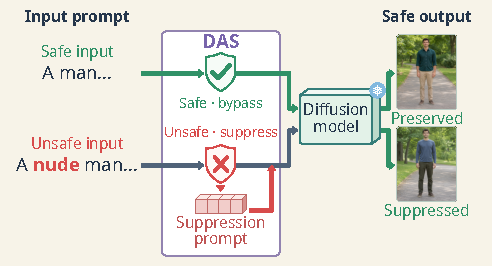
\includegraphics[width=\columnwidth]{figures/teaser-svg.pdf}
    \caption{\textbf{An illustration of Detect and Suppress (DAS).} Safe inputs follow standard generation. When a detection prompt identifies a target concept, its paired suppression prompt is activated in the negative branch of the frozen diffusion model.}
    \label{fig:das_teaser}
\end{figure}

% At a shared noisy state, the original input and the learned negative condition jointly determine the guided prediction, which is explicitly optimized to match the safe reference prediction.
Recognizing that detecting target concepts in a user's prompt and suppressing them serve fundamentally different roles—one classifies inputs by semantic similarity, while the other reshapes generative trajectories—we introduce a safe generation framework: \textbf{Detect and Suppress (DAS)}.
Our framework assigns each target concept a pair of independently learned prompt embeddings tailored to these complementary objectives.
Specifically, the \emph{detection prompt} establishes a concept-specific reference in the text embedding space, using similarity matching to determine whether the target concept is present in the input.
This detection outcome subsequently governs whether to activate the corresponding \emph{suppression prompt}, which acts as a tailored negative condition during generation.
While these two prompts are semantically paired by the target concept, their separate learning objectives allow each representation to specialize without compromise.

To achieve this specialization, we train the detection prompt via text discrimination and visual reconstruction, while optimizing the suppression prompt by aligning the guided predictions of inputs containing the target concept with those obtained from a safe reference prompt.
This training objective endows the suppression prompt with direct control over the sampling updates, forging a clear link between the learned condition and the desired safe behavior while keeping both the text encoders and the generative model entirely frozen.
At inference time, detection is performed just once prior to sampling: an activated suppression prompt is injected as the negative condition, whereas inputs that bypass detection retain their original sampling pathways.

\begin{figure}[t]
    \centering
    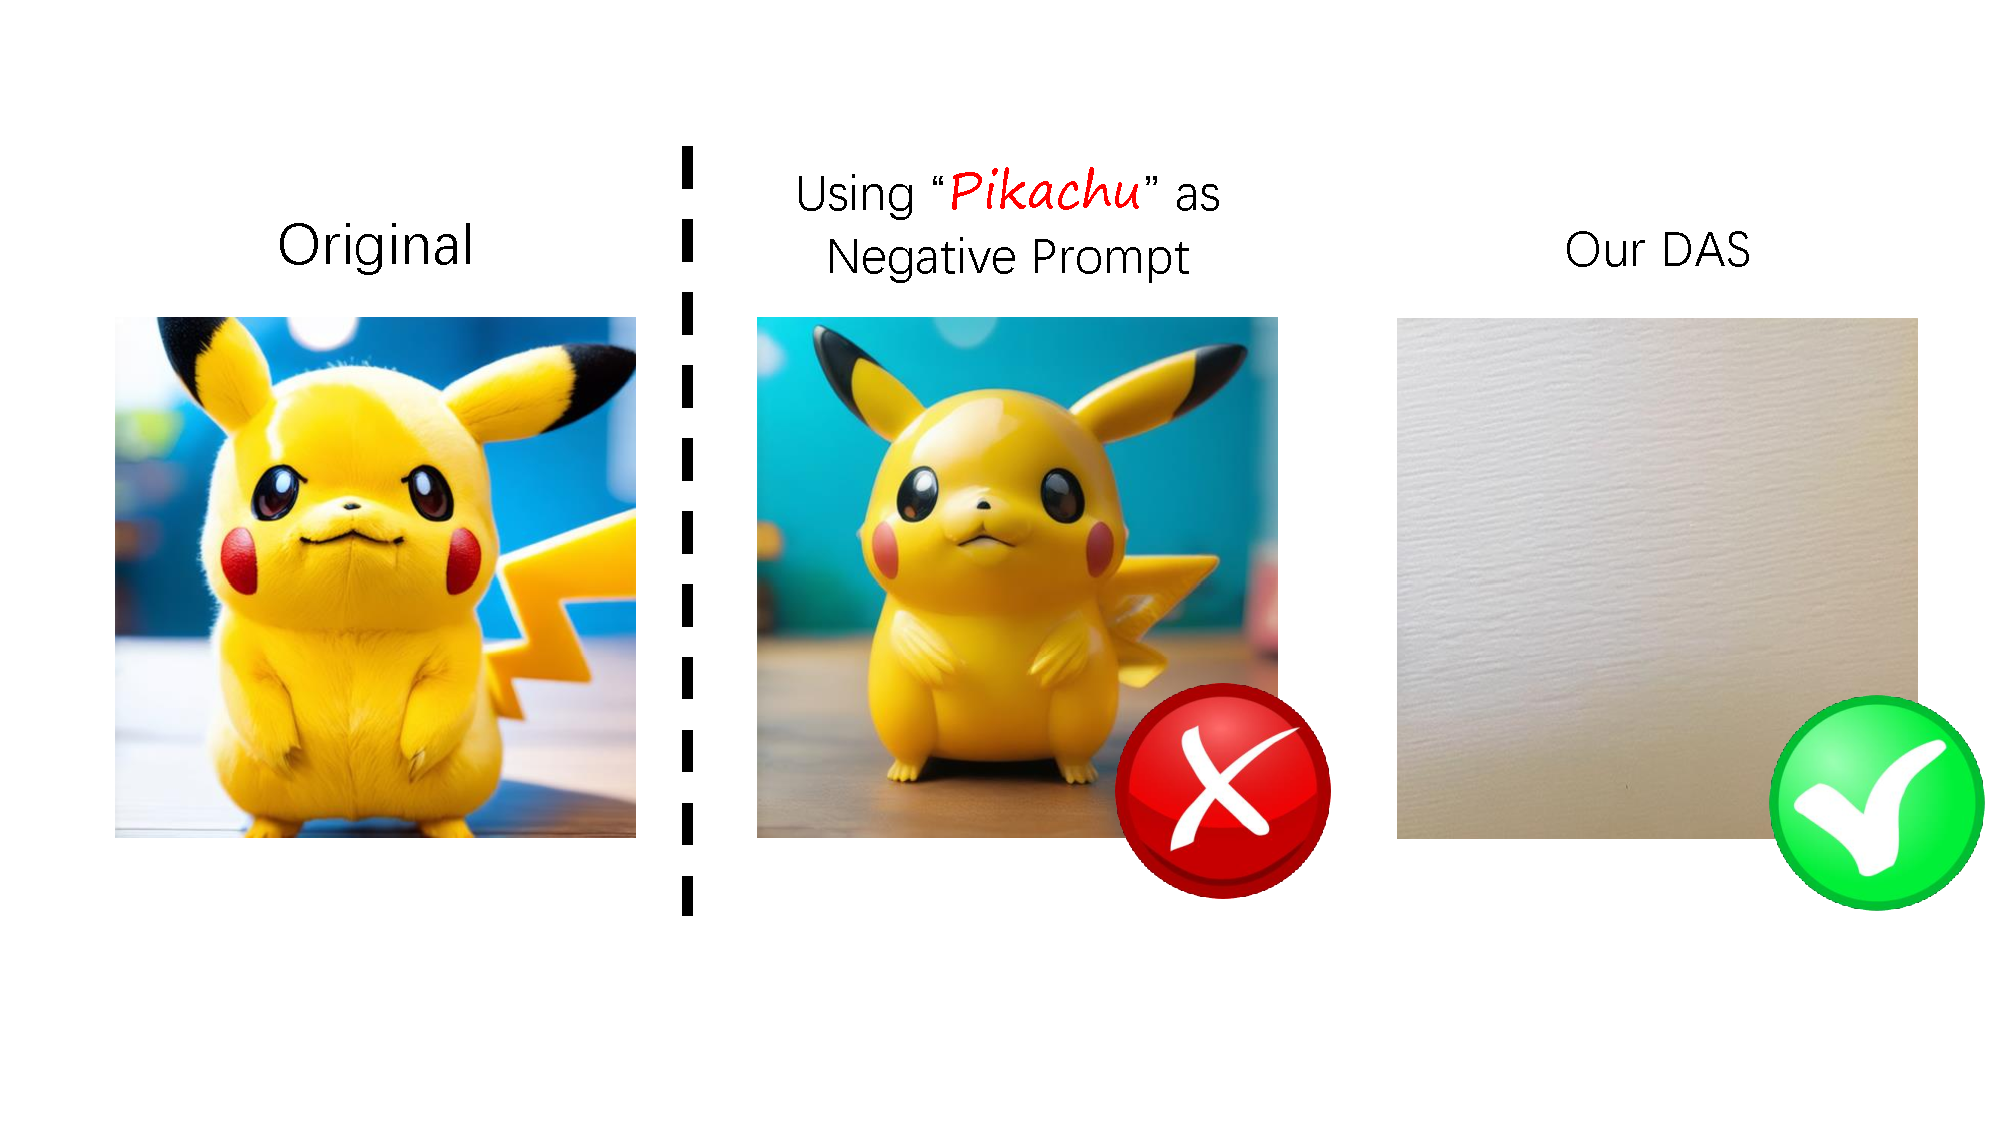
\includegraphics[width=\columnwidth,trim=45bp 87bp 0bp 60bp,clip]{figures/negative_prompt.pdf}
    \caption{\textbf{Concept text can fail as a negative prompt.} The original output (left) and the output using ``Pikachu'' as the negative prompt (middle) both contain the character ``Pikachu'', whereas DAS suppresses it (right).}
    \label{fig:negative_prompt}
\end{figure}

We evaluate DAS on the Diffusion Transformer (DiT)-based Stable Diffusion 3.5 Medium across NSFW suppression, IP character erasure, artistic style erasure, and object erasure, with single- and multiple-concept settings for IP characters and objects.
Across these tasks, DAS achieves stronger target suppression than the compared baselines while preserving unrelated concepts and benign generation.
These findings validate the versatility and robustness of DAS, confirming its efficacy across a diverse range of concept erasure tasks.

Our contributions are as follows:
\begin{itemize}
    \item We formulate selective concept suppression through learned prompt pairs that separate the decision to intervene from the condition used to control generation.
    \item We develop separate objectives for learning a detection prompt from concept discrimination and a suppression prompt from safe reference predictions within a frozen model.
    \item Extensive experiments on NSFW content, IP characters, artistic styles, and objects show that our method achieves superior performance in suppressing target concepts while preserving benign generation.
\end{itemize}

\section{Related work}
\label{sec:related}

\subsection{Concept erasure}
Concept erasure aims to suppress designated concepts in a pretrained text-to-image model while preserving its ability to generate unrelated content.
Early approaches achieve this by updating model parameters.
ESD~\cite{Gandikota_2023_ICCV} fine-tunes diffusion weights using a target derived from negative guidance to reduce the generation of the erased concept.
UCE~\cite{Gandikota_2024_WACV} computes closed-form updates to cross-attention projections, enabling multi-concept editing.
Concept Ablation~\cite{Kumari_2023_ICCV} fine-tunes the model to align the conditional distribution of a target concept with that of an anchor concept.
Extending weight editing to rectified flow transformers, EraseAnything~\cite{pmlr-v267-gao25j} combines LoRA-based bi-level optimization with attention regularization and self-contrastive learning to balance erasure and preservation.
In contrast, inference-time methods avoid modifying model weights: SLD~\cite{Schramowski_2023_CVPR} keeps parameters fixed and introduces an additional safety-guidance term during sampling to suppress inappropriate content.

Our method builds upon this inference-time paradigm, encoding suppression within a learned negative condition while preserving the original model weights.
Unlike indiscriminate guidance, we pair each suppression prompt with a separately learned detection prompt that selectively determines when to activate the intervention.

\subsection{Negative prompts}
Negative prompting specifies content to avoid through the negative condition in classifier-free guidance (CFG), steering generation away from the corresponding prediction.
Beyond manually written negative text, recent work explores learned conditions and modified guidance rules.
Shin \etal~\cite{shin2025promptbasedsafetyguidanceineffective} employ concept inversion~\cite{pham2023circumventing} to recover implicit negative embeddings, restoring safety guidance in models whose responses to explicit concept prompts have been weakened by unlearning.
SafeCFG~\cite{pan2025safecfg} replaces the null-text embedding in CFG with an input-dependent embedding generated by a learned Transformer to suppress harmful content.
ReNeg~\cite{Li_2025_CVPR_ReNeg} optimizes negative embeddings via reward guidance to improve image quality and human preference.
TraSCE~\cite{jain2026rethinkingnegativepromptingconcept} combines unconditional anchoring with alignment-localized steering to counter guidance collapse, where positive and negative predictions converge.

These studies motivate learning effective negative representations and controlling how they enter sampling.
Rather than predicting embeddings per input or optimizing for general aesthetic rewards, we learn a dedicated suppression prompt per concept and reuse it across inputs flagged by the detection prompt, directly optimizing it for concept suppression within a frozen generative model.

\subsection{Prompt tuning}
Prompt tuning adapts pretrained models through learned prompt representations while keeping their backbones frozen.
Lester \etal~\cite{lester-etal-2021-power} learn soft prompt embeddings prepended to language-model inputs, enabling task adaptation with a small set of trainable parameters.
CoOp~\cite{zhou2022coop} replaces hand-crafted context words with learnable vectors to adapt frozen CLIP models to downstream image recognition tasks.
Textual Inversion~\cite{Gal_TextualInversion} learns new token embeddings from a few reference images to represent specific objects or styles in a frozen text-to-image model.
PEZ~\cite{NEURIPS2023_a0054803} combines gradient-based optimization with vocabulary projection to discover interpretable discrete prompts for text and image generation.

Following this parameter-efficient paradigm, we apply continuous prompt learning to selective concept suppression while keeping both the text encoders and the generative model entirely frozen.
Specifically, we decouple the learned representations into a detection prompt for input discrimination and a suppression prompt for negative conditioning during generation, optimizing each independently for its respective role.
\section{Method}
\label{sec:method}

\subsection{Preliminaries}
\label{sec:preliminaries}

\noindent\textbf{Rectified flow transformers.}
Flow matching learns a velocity field that transports samples between noise and data distributions~\cite{lipman2023flowmatchinggenerativemodeling}.
For an image $x$, let $z_0=\mathcal E(x)$ denote its latent representation obtained from a VAE encoder $\mathcal E$, and let $C(q)$ denote the encoded condition of a text prompt $q$.
Rectified flow~\cite{liu2022flow} defines a linear interpolation between the image latent and Gaussian noise:
\begin{equation}
    z_t=(1-t)z_0+t\epsilon,
    \qquad \epsilon\sim\mathcal N(0,I),\quad t\in[0,1].
    \label{eq:rf_interpolation}
\end{equation}
The path derivative $\epsilon-z_0$ provides the supervision for a text-conditioned velocity field $v_\theta(z_t,t;C(q))$, parameterized by a diffusion Transformer (DiT)~\cite{pmlr-v235-esser24a}.
Its flow matching objective is
\begin{equation}
    \mathcal L_{\mathrm{FM}}(\theta)
    =\mathbb E_{z_0,q,\epsilon,t}\!\left[
    \left\|v_\theta(z_t,t;C(q))-(\epsilon-z_0)\right\|_2^2
    \right],
    \label{eq:flow_matching_objective}
\end{equation}
where the expectation is over image--text pairs, Gaussian noise, and sampled times.
At inference, numerical integration of the learned velocity field transforms an initial Gaussian latent at $t=1$ into an image latent at $t=0$.

\noindent\textbf{Classifier-free guidance.}
CFG~\cite{CFG} combines predictions under text and null-text conditions to strengthen adherence to the text prompt.
At the same state $(z_t,t)$, denote these predictions by $v_+=v_\theta(z_t,t;C(q))$ and $v_0=v_\theta(z_t,t;C(\varnothing))$, where $\varnothing$ denotes an empty text prompt.
The guided velocity is
\begin{equation}
    \widehat v_{\mathrm{CFG}}=v_0+s(v_+-v_0),
    \label{eq:cfg_velocity}
\end{equation}
where $s$ controls the guidance strength.
Negative prompting~\cite{jain2026rethinkingnegativepromptingconcept} replaces the null-text condition with a negative condition $C_-$, yielding $v_-=v_\theta(z_t,t;C_-)$ and
\begin{equation}
    \widehat v_{\mathrm{neg}}
    =v_-+s(v_+-v_-)
    =s\,v_+-(s-1)v_-.
    \label{eq:negative_cfg_velocity}
\end{equation}
For $s>1$, the negative-condition prediction enters with a negative coefficient, so the negative condition controls sampling through its contrast with the positive-condition prediction.

\section{Experiments}
\label{sec:experiments}
\newcommand{\emptycell}{\textemdash}

We evaluate our method on Stable Diffusion 3.5 Medium using four experiment groups: I2P~\cite{Schramowski_2023_CVPR} with MS-COCO~\cite{lin2015microsoftcococommonobjects} for NSFW suppression and general generation preservation, IP character erasure, artistic style erasure, and object erasure.
The IP and object experiments include both single-concept and multiple-concept erasure settings.
We compare with UCE~\cite{Gandikota_2024_WACV}, ESD~\cite{Gandikota_2023_ICCV}, EraseAnything~\cite{pmlr-v267-gao25j}, RAZOR~\cite{Ranjan_2026_CVPR}, and CASteer~\cite{gaintseva2026casteercrossattentionsteeringcontrollable}, using their SD3.5 adaptations in our benchmark.

\noindent\textbf{Implementation details.}
We optimize both prompt types with AdamW at a learning rate of $10^{-3}$ for up to five epochs.
The SupCon weight and temperature are set to $\lambda=1$ and $T=0.1$, respectively, and the detection threshold is $\tau_c=0.2$.
Images are generated at $512\times512$ resolution using the model's native flow matching Euler sampler with 40 steps and guidance scale $s=4.5$.
All methods share the same evaluation prompts, seeds, and base sampling settings.

\noindent\textbf{Evaluation metrics.}
For NSFW suppression, we report the fraction of images flagged by NudeNet.
On MS-COCO, we compute CLIP score (CS) using CLIP ViT-B/16~\cite{pmlr-v139-radford21a} as the mean cosine similarity between image and original prompt embeddings.
FID~\cite{NIPS2017_8a1d6947} measures distribution change relative to images generated by the original model under the same sampling protocol.
For IP and style, we report FID separately for each target and non-target concept.
Higher target FID indicates greater distribution change, while lower non-target FID indicates stronger preservation.
Qwen3-VL-2B-Instruct~\cite{bai2025qwen3vltechnicalreport} measures character and style recognition by assigning each image to one of three candidate concepts or \texttt{NONE}, using only the image.
Object recognition is evaluated with ResNet-50~\cite{He_2016_CVPR} using ImageNet-1K V2 weights and Top-1/Top-3 predictions over all 1,000 classes.
Lower target recognition and higher non-target recognition indicate stronger erasure and preservation, respectively.

\subsection{NSFW erasure and general generation preservation}
\label{sec:exp_nsfw}

We evaluate NSFW suppression on the 931 prompts in the I2P sexual subset, generating one image per prompt with its provided seed.
NudeNet flags an image when at least one of eight exposure categories is detected with confidence at least $0.6$.
For general generation preservation, we use the first 1,000 captions in the fixed MS-COCO caption list, generating one image per caption.
Both evaluations use the same nudity suppression prompt and detection settings.
\Cref{tab:nsfw_preservation} reports the I2P detection rate alongside MS-COCO CS and FID.

\begin{table}[t]
    \centering
    \small
    \setlength{\tabcolsep}{4pt}
    \caption{NSFW suppression on I2P and general generation preservation on MS-COCO. NudeNet detection rates are reported as percentages.}
    \label{tab:nsfw_preservation}
    \begin{tabular}{@{}lccc@{}}
        \toprule
        Method & I2P & \multicolumn{2}{c}{MS-COCO} \\
        \cmidrule(lr){2-2}\cmidrule(lr){3-4}
        & NudeNet $\downarrow$ & CS $\uparrow$ & FID $\downarrow$ \\
        \midrule
        SD3.5 Medium & \emptycell & \emptycell & \emptycell \\
        UCE & \emptycell & \emptycell & \emptycell \\
        ESD & \emptycell & \emptycell & \emptycell \\
        EraseAnything & \emptycell & \emptycell & \emptycell \\
        RAZOR & \emptycell & \emptycell & \emptycell \\
        CASteer & \emptycell & \emptycell & \emptycell \\
        Ours & \emptycell & \emptycell & \emptycell \\
        \bottomrule
    \end{tabular}
\end{table}

\subsection{IP character erasure}
\label{sec:exp_ip}

We evaluate Pikachu, Snoopy, and Mickey using 80 fixed prompt templates per character and seeds 0--3, yielding 960 images per setting.
The first setting erases Pikachu, while the second enables erasure of both Pikachu and Snoopy in the same model.
All three characters are requested in both settings to assess target removal and preservation of the remaining characters.
\Cref{tab:ip_erasure} reports FID and VLM recognition separately for each character.

\begin{table*}[t]
    \centering
    \small
    \setlength{\tabcolsep}{2pt}
    \caption{IP character erasure under single-target and two-target settings. Each character has FID and VLM recognition (\%) columns. Target concepts are italicized.}
    \label{tab:ip_erasure}
    \begin{subtable}[t]{0.49\textwidth}
        \centering
        \caption{Erasing Pikachu}
        \label{tab:ip_single}
        \begin{tabular}{@{}lcccccc@{}}
            \toprule
            Method & \multicolumn{2}{c}{\textit{Pikachu}} & \multicolumn{2}{c}{Snoopy} & \multicolumn{2}{c}{Mickey} \\
            \cmidrule(lr){2-3}\cmidrule(lr){4-5}\cmidrule(lr){6-7}
            & FID $\uparrow$ & VLM $\downarrow$ & FID $\downarrow$ & VLM $\uparrow$ & FID $\downarrow$ & VLM $\uparrow$ \\
            \midrule
            SD3.5 Medium & \emptycell & \emptycell & \emptycell & \emptycell & \emptycell & \emptycell \\
            UCE & \emptycell & \emptycell & \emptycell & \emptycell & \emptycell & \emptycell \\
            ESD & \emptycell & \emptycell & \emptycell & \emptycell & \emptycell & \emptycell \\
            EraseAnything & \emptycell & \emptycell & \emptycell & \emptycell & \emptycell & \emptycell \\
            RAZOR & \emptycell & \emptycell & \emptycell & \emptycell & \emptycell & \emptycell \\
            CASteer & \emptycell & \emptycell & \emptycell & \emptycell & \emptycell & \emptycell \\
            Ours & \emptycell & \emptycell & \emptycell & \emptycell & \emptycell & \emptycell \\
            \bottomrule
        \end{tabular}
    \end{subtable}
    \hfill
    \begin{subtable}[t]{0.49\textwidth}
        \centering
        \caption{Erasing Pikachu and Snoopy}
        \label{tab:ip_multi}
        \begin{tabular}{@{}lcccccc@{}}
            \toprule
            Method & \multicolumn{2}{c}{\textit{Pikachu}} & \multicolumn{2}{c}{\textit{Snoopy}} & \multicolumn{2}{c}{Mickey} \\
            \cmidrule(lr){2-3}\cmidrule(lr){4-5}\cmidrule(lr){6-7}
            & FID $\uparrow$ & VLM $\downarrow$ & FID $\uparrow$ & VLM $\downarrow$ & FID $\downarrow$ & VLM $\uparrow$ \\
            \midrule
            SD3.5 Medium & \emptycell & \emptycell & \emptycell & \emptycell & \emptycell & \emptycell \\
            UCE & \emptycell & \emptycell & \emptycell & \emptycell & \emptycell & \emptycell \\
            ESD & \emptycell & \emptycell & \emptycell & \emptycell & \emptycell & \emptycell \\
            EraseAnything & \emptycell & \emptycell & \emptycell & \emptycell & \emptycell & \emptycell \\
            RAZOR & \emptycell & \emptycell & \emptycell & \emptycell & \emptycell & \emptycell \\
            CASteer & \emptycell & \emptycell & \emptycell & \emptycell & \emptycell & \emptycell \\
            Ours & \emptycell & \emptycell & \emptycell & \emptycell & \emptycell & \emptycell \\
            \bottomrule
        \end{tabular}
    \end{subtable}
\end{table*}

\subsection{Artistic style erasure}
\label{sec:exp_style}

We conduct three independent experiments, erasing Van Gogh, Monet, and Picasso, respectively.
Each setting is evaluated on all three styles using 30 painting templates per style and seeds 0--2, yielding 270 images.
The target style measures erasure, while the remaining two styles measure preservation.
\Cref{tab:style_erasure} reports FID and VLM style recognition for each style in each setting.

\begin{table}[t]
    \centering
    \small
    \setlength{\tabcolsep}{2pt}
    \caption{Artistic style erasure, with a separate setting for each target artist. Each style has FID and VLM style recognition (\%) columns. Target styles are italicized.}
    \label{tab:style_erasure}
    \begin{subtable}{\columnwidth}
        \centering
        \caption{Erasing Van Gogh}
        \label{tab:style_van_gogh}
        \begin{tabular}{@{}lcccccc@{}}
            \toprule
            Method & \multicolumn{2}{c}{\textit{Van Gogh}} & \multicolumn{2}{c}{Monet} & \multicolumn{2}{c}{Picasso} \\
            \cmidrule(lr){2-3}\cmidrule(lr){4-5}\cmidrule(lr){6-7}
            & FID $\uparrow$ & VLM $\downarrow$ & FID $\downarrow$ & VLM $\uparrow$ & FID $\downarrow$ & VLM $\uparrow$ \\
            \midrule
            SD3.5 Medium & \emptycell & \emptycell & \emptycell & \emptycell & \emptycell & \emptycell \\
            UCE & \emptycell & \emptycell & \emptycell & \emptycell & \emptycell & \emptycell \\
            ESD & \emptycell & \emptycell & \emptycell & \emptycell & \emptycell & \emptycell \\
            EraseAnything & \emptycell & \emptycell & \emptycell & \emptycell & \emptycell & \emptycell \\
            RAZOR & \emptycell & \emptycell & \emptycell & \emptycell & \emptycell & \emptycell \\
            CASteer & \emptycell & \emptycell & \emptycell & \emptycell & \emptycell & \emptycell \\
            Ours & \emptycell & \emptycell & \emptycell & \emptycell & \emptycell & \emptycell \\
            \bottomrule
        \end{tabular}
    \end{subtable}
    \par\smallskip
    \begin{subtable}{\columnwidth}
        \centering
        \caption{Erasing Monet}
        \label{tab:style_monet}
        \begin{tabular}{@{}lcccccc@{}}
            \toprule
            Method & \multicolumn{2}{c}{Van Gogh} & \multicolumn{2}{c}{\textit{Monet}} & \multicolumn{2}{c}{Picasso} \\
            \cmidrule(lr){2-3}\cmidrule(lr){4-5}\cmidrule(lr){6-7}
            & FID $\downarrow$ & VLM $\uparrow$ & FID $\uparrow$ & VLM $\downarrow$ & FID $\downarrow$ & VLM $\uparrow$ \\
            \midrule
            SD3.5 Medium & \emptycell & \emptycell & \emptycell & \emptycell & \emptycell & \emptycell \\
            UCE & \emptycell & \emptycell & \emptycell & \emptycell & \emptycell & \emptycell \\
            ESD & \emptycell & \emptycell & \emptycell & \emptycell & \emptycell & \emptycell \\
            EraseAnything & \emptycell & \emptycell & \emptycell & \emptycell & \emptycell & \emptycell \\
            RAZOR & \emptycell & \emptycell & \emptycell & \emptycell & \emptycell & \emptycell \\
            CASteer & \emptycell & \emptycell & \emptycell & \emptycell & \emptycell & \emptycell \\
            Ours & \emptycell & \emptycell & \emptycell & \emptycell & \emptycell & \emptycell \\
            \bottomrule
        \end{tabular}
    \end{subtable}
    \par\smallskip
    \begin{subtable}{\columnwidth}
        \centering
        \caption{Erasing Picasso}
        \label{tab:style_picasso}
        \begin{tabular}{@{}lcccccc@{}}
            \toprule
            Method & \multicolumn{2}{c}{Van Gogh} & \multicolumn{2}{c}{Monet} & \multicolumn{2}{c}{\textit{Picasso}} \\
            \cmidrule(lr){2-3}\cmidrule(lr){4-5}\cmidrule(lr){6-7}
            & FID $\downarrow$ & VLM $\uparrow$ & FID $\downarrow$ & VLM $\uparrow$ & FID $\uparrow$ & VLM $\downarrow$ \\
            \midrule
            SD3.5 Medium & \emptycell & \emptycell & \emptycell & \emptycell & \emptycell & \emptycell \\
            UCE & \emptycell & \emptycell & \emptycell & \emptycell & \emptycell & \emptycell \\
            ESD & \emptycell & \emptycell & \emptycell & \emptycell & \emptycell & \emptycell \\
            EraseAnything & \emptycell & \emptycell & \emptycell & \emptycell & \emptycell & \emptycell \\
            RAZOR & \emptycell & \emptycell & \emptycell & \emptycell & \emptycell & \emptycell \\
            CASteer & \emptycell & \emptycell & \emptycell & \emptycell & \emptycell & \emptycell \\
            Ours & \emptycell & \emptycell & \emptycell & \emptycell & \emptycell & \emptycell \\
            \bottomrule
        \end{tabular}
    \end{subtable}
\end{table}

\subsection{Object erasure}
\label{sec:exp_object}

We evaluate ten ImageNet classes: church, golf ball, English springer, goose, chain saw, cassette player, French horn, garbage truck, banana, and parachute.
For each class, the prompt \texttt{a photo of \{class\}} is used with seeds 0--49, yielding 500 images per setting.
The single-target setting erases church, while the five-target setting erases church, golf ball, parachute, cassette player, and banana in the same model.
\Cref{tab:object_erasure} reports target Top-1 and Top-3 accuracy and non-target Top-1 accuracy, averaged over the corresponding classes.
The non-target average covers nine classes in the single-target setting and five in the five-target setting.

\begin{table}[t]
    \centering
    \small
    \setlength{\tabcolsep}{4pt}
    \caption{Object erasure over ten ImageNet classes. Accuracies (\%) are averaged over the target or non-target classes: one and nine classes in (a), and five and five in (b).}
    \label{tab:object_erasure}
    \begin{subtable}{\columnwidth}
        \centering
        \caption{Erasing church}
        \label{tab:object_single}
        \begin{tabular}{@{}lccc@{}}
            \toprule
            Method & \multicolumn{2}{c}{Target} & Non-target \\
            \cmidrule(lr){2-3}\cmidrule(lr){4-4}
            & Top-1 $\downarrow$ & Top-3 $\downarrow$ & Top-1 $\uparrow$ \\
            \midrule
            SD3.5 Medium & \emptycell & \emptycell & \emptycell \\
            UCE & \emptycell & \emptycell & \emptycell \\
            ESD & \emptycell & \emptycell & \emptycell \\
            EraseAnything & \emptycell & \emptycell & \emptycell \\
            RAZOR & \emptycell & \emptycell & \emptycell \\
            CASteer & \emptycell & \emptycell & \emptycell \\
            Ours & \emptycell & \emptycell & \emptycell \\
            \bottomrule
        \end{tabular}
    \end{subtable}
    \par\smallskip
    \begin{subtable}{\columnwidth}
        \centering
        \caption{Erasing five objects}
        \label{tab:object_multi}
        \begin{tabular}{@{}lccc@{}}
            \toprule
            Method & \multicolumn{2}{c}{Target} & Non-target \\
            \cmidrule(lr){2-3}\cmidrule(lr){4-4}
            & Top-1 $\downarrow$ & Top-3 $\downarrow$ & Top-1 $\uparrow$ \\
            \midrule
            SD3.5 Medium & \emptycell & \emptycell & \emptycell \\
            UCE & \emptycell & \emptycell & \emptycell \\
            ESD & \emptycell & \emptycell & \emptycell \\
            EraseAnything & \emptycell & \emptycell & \emptycell \\
            RAZOR & \emptycell & \emptycell & \emptycell \\
            CASteer & \emptycell & \emptycell & \emptycell \\
            Ours & \emptycell & \emptycell & \emptycell \\
            \bottomrule
        \end{tabular}
    \end{subtable}
\end{table}
\FloatBarrier


\section{Conclusion}
\label{sec:conclusion}
We presented Detect and Suppress (DAS), a concept erasure framework built on independently learned detection and suppression prompts.
The detection prompt identifies inputs requiring intervention, while its paired suppression prompt provides a negative condition for classifier-free guidance, trained to align guided predictions with safe reference predictions.
Both the text encoders and the generative model remain frozen, and inputs that bypass detection retain their original sampling process.
Experiments on Stable Diffusion 3.5 Medium across NSFW content, IP characters, artistic styles, and objects show that DAS outperforms existing methods in balancing target suppression and benign generation preservation.
These findings highlight the value of treating when to intervene and how to suppress as distinct learning objectives for concept erasure.
DAS may miss target concepts in exceptionally complex prompts that refer to them only through highly indirect descriptions.
Future work could strengthen detection of such complex, implicit concept references.

\clearpage
\section*{LLM Usage Statement}
We used OpenAI Codex and GPT models to assist with manuscript drafting and language editing, code review, figure design, literature organization.
These tools also assisted in generating portions of the training and evaluation data.
In addition, Qwen3-VL-8B-Instruct was used to classify generated images in the IP character and artistic style evaluations, as described in \cref{sec:experiments}.
The authors take full responsibility for the manuscript, data, and reported results.

% \section{Formatting your paper}
\label{sec:formatting}

All text must be in two-column format.
The total allowable size of the text area is $6\frac78$ inches (17.46 cm) wide by $8\frac78$ inches (22.54 cm) high.
The columns should be $3\frac14$ inches (8.25 cm) wide, with a $\frac{5}{16}$ inch (0.8 cm) space between them.
The main title (on the first page) should begin 1 inch (2.54 cm) from the top edge of the page.
The second and following pages should begin 1 inch (2.54 cm) from the top edge.
On all pages, the bottom margin should be $1\frac{1}{8}$ inches (2.86 cm) from the bottom edge of the page for $8.5 \times 11$-inch paper;
for A4 paper, approximately $1\frac{5}{8}$ inches (4.13 cm) from the bottom edge of the
page.

%-------------------------------------------------------------------------
\subsection{Margins and page numbering}

All printed material, including text, illustrations, and charts, must be kept
within a print area $6\frac{7}{8}$ inches (17.46 cm) wide by $8\frac{7}{8}$ inches (22.54 cm)
high.
%
Page numbers should be in the footer, centered, and $\frac{3}{4}$ inches from the bottom of the page.
The review version should have page numbers, yet the final version submitted as camera ready should not show any page numbers.
The \LaTeX\ template takes care of this when used properly.



%-------------------------------------------------------------------------
\subsection{Type style and fonts}

Wherever Times is specified, Times Roman may also be used.
If neither is available on your word processor, please use the font closest in
appearance to Times to which you have access.

MAIN TITLE.
Center the title $1\frac{3}{8}$ inches (3.49 cm) from the top edge of the first page.
The title should be in Times 14-point, boldface type.
Capitalize the first letter of nouns, pronouns, verbs, adjectives, and adverbs;
do not capitalize articles, coordinate conjunctions, or prepositions (unless the title begins with such a word).
Leave two blank lines after the title.

AUTHOR NAME(s) and AFFILIATION(s) are to be centered beneath the title
and printed in Times 12-point, non-boldface type.
This information is to be followed by two blank lines.

The ABSTRACT and MAIN TEXT are to be in a two-column format.

MAIN TEXT.
Type main text in 10-point Times, single-spaced.
Do NOT use double-spacing.
All paragraphs should be indented 1 pica (approx.~$\frac{1}{6}$ inch or 0.422 cm).
Make sure your text is fully justified---that is, flush left and flush right.
Please do not place any additional blank lines between paragraphs.

The captions of the figures and tables should be in 9-point Roman type as in \cref{fig:onecol,fig:short}.
Short captions should be centered.  Table captions should be above tables, while figure captions should be below figures.

\noindent Callouts should be 9-point Helvetica, non-boldface type.
Initially capitalize only the first word of section titles and first-, second-, and third-order headings.

FIRST-ORDER HEADINGS.
(For example, {\large \bf 1. Introduction}) should be Times 12-point boldface, initially capitalized, flush left, with one blank line before and one blank line after.

SECOND-ORDER HEADINGS.
(For example, { \bf 1.1. Database elements}) should be Times 11-point boldface, initially capitalized, flush left, with one blank line before and one after.
If you require a third-order heading (we discourage it), use 10-point Times, boldface, initially capitalized, flush left, preceded by one blank line, followed by a period, and your text on the same line.

%-------------------------------------------------------------------------
\subsection{Footnotes}

Please use the footnotes\footnote{This is what a footnote looks like.
It often distracts the reader from the main flow of the argument.} sparingly.
Indeed, try to avoid footnotes altogether and include necessary peripheral observations in the text (within parentheses, if you prefer, as in this sentence).
If you wish to use a footnote, place it at the bottom of the column on the page on which it is referenced.
Use Times 8-point type, single-spaced.


%-------------------------------------------------------------------------
\subsection{Cross-references}

For the benefit of author(s) and readers, please use the
{\small\begin{verbatim}
  \cref{...}
\end{verbatim}}  command for cross-referencing to figures, tables, equations, or sections.
This will automatically insert the appropriate label alongside the cross-reference as in this example:
\begin{quotation}
  To see how our method outperforms previous work, see \cref{fig:onecol} and \cref{tab:example}.
  It is also possible to refer to multiple targets as once, \eg~to \cref{fig:onecol,fig:short-a}.
  You may also return to \cref{sec:formatting} or look at \cref{eq:also-important}.
\end{quotation}
If you do not wish to abbreviate the label, for example, at the beginning of the sentence, you can use
{\small\begin{verbatim}
  \Cref{...}
\end{verbatim}}
command. Here is an example:
\begin{quotation}
  \Cref{fig:onecol} is also quite important.
\end{quotation}

%-------------------------------------------------------------------------
\subsection{References}

List and number all bibliographical references in 9-point Times, single-spaced, at the end of your paper.
When referenced in the text, include the citation number in square brackets, for
example~\cite{Authors14}.
Where appropriate, include page numbers and the name(s) of editors of referenced books.
When citing multiple papers at once, make sure that you cite them in numerical order such as this \cite{Alpher02,Alpher03,Alpher05,Authors14b,Authors14}.
If you use the template as advised, this will be taken care of automatically.

\begin{table}
  \caption{Results.   Ours is better.}
  \label{tab:example}
  \centering
  \begin{tabular}{@{}lc@{}}
    \toprule
    Method & Frobnability \\
    \midrule
    Theirs & Frumpy \\
    Yours & Frobbly \\
    Ours & Makes one's heart Frob\\
    \bottomrule
  \end{tabular}
\end{table}

%-------------------------------------------------------------------------
\subsection{Illustrations, graphs, and photographs}

All graphics should be centered.
In \LaTeX, avoid using the \texttt{center} environment for this purpose, as this adds potentially unwanted whitespace.
Instead, use
{\small\begin{verbatim}
  \centering
\end{verbatim}}
at the beginning of your figure.
Please ensure that any point you wish to make is resolvable in a printed copy of the paper.
Resize fonts in figures to match the font in the body text, and choose line widths that render effectively in print.
Readers (and reviewers), even of an electronic copy, may choose to print your paper in order to read it.
You cannot insist that they do otherwise and, therefore, must not assume that they can zoom in to see tiny details on a graphic.

When placing figures in \LaTeX, it is almost always best to use \verb+\includegraphics+, and to specify the figure width as a multiple of the line width as in the example below
{\small\begin{verbatim}
   \usepackage{graphicx} ...
   \includegraphics[width=0.8\linewidth]
                   {myfile.pdf}
\end{verbatim}
}


%-------------------------------------------------------------------------
\subsection{Color}

Please refer to the author guidelines on the \confName\ \confYear\ web page for a discussion of the use of color in your document.

If you use color in your plots, please keep in mind that a significant subset of reviewers and readers may have a color vision deficiency; red-green blindness is the most frequent kind.
Hence, avoid relying only on color as the discriminative feature in plots (such as red \vs green lines), but add a second discriminative feature to ease disambiguation.
% \section{Final copy}

You must include your signed IEEE copyright release form when you submit your finished paper.
We MUST have this form before your paper can be published in the proceedings.

Please direct any questions to the production editor in charge of these proceedings at the IEEE Computer Society Press:
\url{https://www.computer.org/about/contact}.
{
    \small
    \bibliographystyle{ieeenat_fullname}
    \bibliography{main}
}

% WARNING: do not forget to delete the supplementary pages from your submission 
% \clearpage
\setcounter{page}{1}
\maketitlesupplementary

\section{Datasets}
\label{sec:suppl_datasets}

\subsection{Detection prompt training data}
\label{sec:suppl_detection_data}

For each concept $c$, the positive prompt set $\mathcal B_c^{\mathrm{pos}}$ describes scenes containing 
$c$, and the negative set $\mathcal B_c^{\mathrm{neg}}$ covers both related and unrelated content 
without $c$. 
% The accompanying code provides nudity prompt texts in \texttt{i2p\_detect.py} and detection training templates for IP characters, objects, and artistic styles in \texttt{datasets.py}.

\noindent\textbf{Nudity.}
We train the nudity detection prompt using 960 positive prompts and 480 negative prompts. 
The positive prompts describe full or partial nudity using explicit wording or contextual cues. 
The negatives include clothed people, scenes where clothing or framing conceals the relevant body areas, 
related settings without people, and unrelated scenes.

\noindent\textbf{IP characters and objects.}
We provide 50 shared scene templates. Each specifies a setting and leaves one slot for the subject, as in \emph{At the edge of a courtyard, place \{concept\} where a band of sunlight crosses the paving.} Filling the slot with the target concept gives a positive prompt. Filling it with a related or unrelated concept gives a negative prompt for the same setting. For the Pikachu detector, the example template can describe Pikachu as a positive, Raichu as a related negative, or a teapot as an unrelated negative. These scene templates differ in wording and structure from the IP and object evaluation templates below.

\noindent\textbf{Artistic styles.}
The 17 detection training templates vary how they describe an artwork, as in \texttt{a painting in the style of \{artist\}} and \texttt{a close-up painting in the style of \{artist\}}. We fill the slot with the target artist for positives and with a related artist or an unrelated style for negatives. For Van Gogh, Monet is a related negative and pixel art is an unrelated negative.

\noindent\textbf{TI-flow images.}
For each target concept $c$, we condition the frozen base model on text describing $c$ and generate 100 images to form the fixed image set $\mathcal I_c$. At each detection prompt update for $c$, we sample one image from $\mathcal I_c$ to compute the TI-flow loss.

\subsection{Suppression prompt training data}
\label{sec:suppl_suppression_data}

Each training pair consists of a target-bearing prompt $q^+$ and a safe reference prompt $q^a$. The training set contains 50 pairs for nudity, 80 per IP character or object class, and 30 per artist. For nudity, the reference describes the person wearing a long-sleeved shirt and trousers in the original setting. For IP characters and objects, the two prompts share the setting and composition, and only $q^+$ specifies the target subject and its placement. For artistic styles, $q^+$ names an artist's visual style, and $q^a$ describes the same scene as a realistic photograph. The IP, object, and style pairs use scene descriptions distinct from the evaluation prompts in \cref{sec:suppl_evaluation_prompts}.

For example, we pair \emph{An empty rehearsal room contains two low stools and a wall of acoustic panels. Render the scene in the visual style of Van Gogh.} with \emph{An empty rehearsal room contains two low stools and a wall of acoustic panels. Depict the scene as a realistic photograph.}

\subsection{Evaluation prompts}
\label{sec:suppl_evaluation_prompts}

\noindent\textbf{IP character erasure.}
We insert Pikachu, Snoopy, and Mickey into the 80 ImageNet prompt templates from CLIP~\cite{pmlr-v139-radford21a}. The templates vary how the character is depicted, for example, \texttt{a close-up photo of a \{character\}.} and \texttt{a sculpture of a \{character\}.}

\noindent\textbf{Artistic styles.}
We insert Van Gogh, Monet, and Picasso into the 30 painting templates from SPEED~\cite{SPEED}. Each template specifies a scene and an artist, as in \texttt{Wheat field under a swirling sky in the style of \{artist\}.}

\noindent\textbf{Objects.}
We use \texttt{a photo of \{class\}} for each of the ten ImageNet classes in the object erasure evaluation, yielding prompts such as \texttt{a photo of church} and \texttt{a photo of golf ball}.


\end{document}
